\section{Equilibrium \& Comparative Statics}
\label{sec:section3} 
\subsection{Stationary Equilibrium and Computation}\label{sec:section3.1} 
Using the framework and results above, I now present a refined definition for stationary market equilibria: 
\begin{definition}
    A Stationary Equilibrium (SE) is a triplet $(\mu^*, \omega^*, \Psi^*)$ such that:
    \begin{enumerate}
        \item $ \mu^*(\theta,b) \text{ attains } V_m(\theta,b),$ for all pairs $\theta, b \in \Theta \times \mathcal{B}_m$, given $\omega^*,\Psi^*$.
        \item $ \omega^*(\theta,b) \text{ attains } V_w(\theta,b),$ for all pairs $\theta, b \in \Theta \times \mathcal{B}_w$, given $\mu^*,\Psi^*$.
        \item $\Psi^*$ satisfies Equations \ref{eq:ss1}, \ref{eq:ss2}, and \ref{eq:ss3} given the strategy profile $(\mu^*, \omega^*)$.
    \end{enumerate} 
\end{definition}

Intuitively, the above definition establishes two requirements that must be satisfied by an equilibrium market configuration. 
Firstly, it must be the case that $\mu^*$ and $\omega^*$ are mutual best responses given the platform state $\Psi^*$ for which, as previously outlined, a necessary and sufficient condition would have them each solve the sex-specific MDP. 
These two conditions alone demand \textit{partially rational expectations}, as per \cite{burdett1997marriage}, since they require agents to play optimally for some fixed steady state $\Psi^*$, imposing rationality on all game aspects other than the platform state dynamics. 
Furthermore, in line with other works in mean-field game theory, a consistency check is imposed by the third condition, such that the platform state to which agents are best-responding with $(\mu^*,\omega^*)$ is sustained as a fixed point under that same strategy profile.

Although formal proofs for the existence and uniqueness of SE are outside the scope of this paper, I rely on numerical procedures\footnote{The code required to reproduce all the analysis presented in what follows is accessible under the GitHub repository \texttt{patohdzs/project-swipe}.} to approximate equilibria under various exogenous settings. 
This approach has been frequently employed by related works \citep[see][]{iyer2014mean, gummadi2011optimal} as it can help uncover insights provided by mean-field models. 
To compute model equilibria, I frame the recurrence relation presented in \autoref{prop:recurrence relation}, as well as Equations \ref{eq:ss1}, \ref{eq:ss2}, and \ref{eq:ss3}, as a system of $2(|\mathcal{B}_m|+|\mathcal{B}_w|+1)$ non-linear equations, and solve this using a modified version of the hybrid Powell method, as implemented by the MINPACK 1 routine \citep{more1980user}. 
In what follows, I present SE results for a number of comparative statics experiments. 
For all of these, the exogenous settings used to calibrate the model are provided in \autoref{appx: c}, and convergence of numerical procedures was assured by computing the squared loss of the above system, which was exactly equal to zero in all cases (although the runtime required for convergence varied slightly across experiments).

\subsection{Best Response Analysis}\label{sec:section3.2} 
Using the computational procedures outlined above, a number of insights can be uncovered related to how exogenous parameters affect an agent's optimal swiping behaviour. 
The first parameter I analyse is the discount factor, which represents the probability of remaining inside the platform for an additional time period, but is often interpreted as the representative agent's patience level.
To determine the effects of changes in the discount factor, I computed the best-response policy over a range of different values for $\delta$ (using an arbitrary set of exogenous parameters), with results shown in \autoref{fig:discount-cs}. 
Evidently, as the agent becomes less patient, they `lower their standards' for potential matches in the platform, shifting their swiping curve downwards. 

\begin{figure}[ht] 
    \centering
    \caption{Comparative Statics on the Discount Factor}
    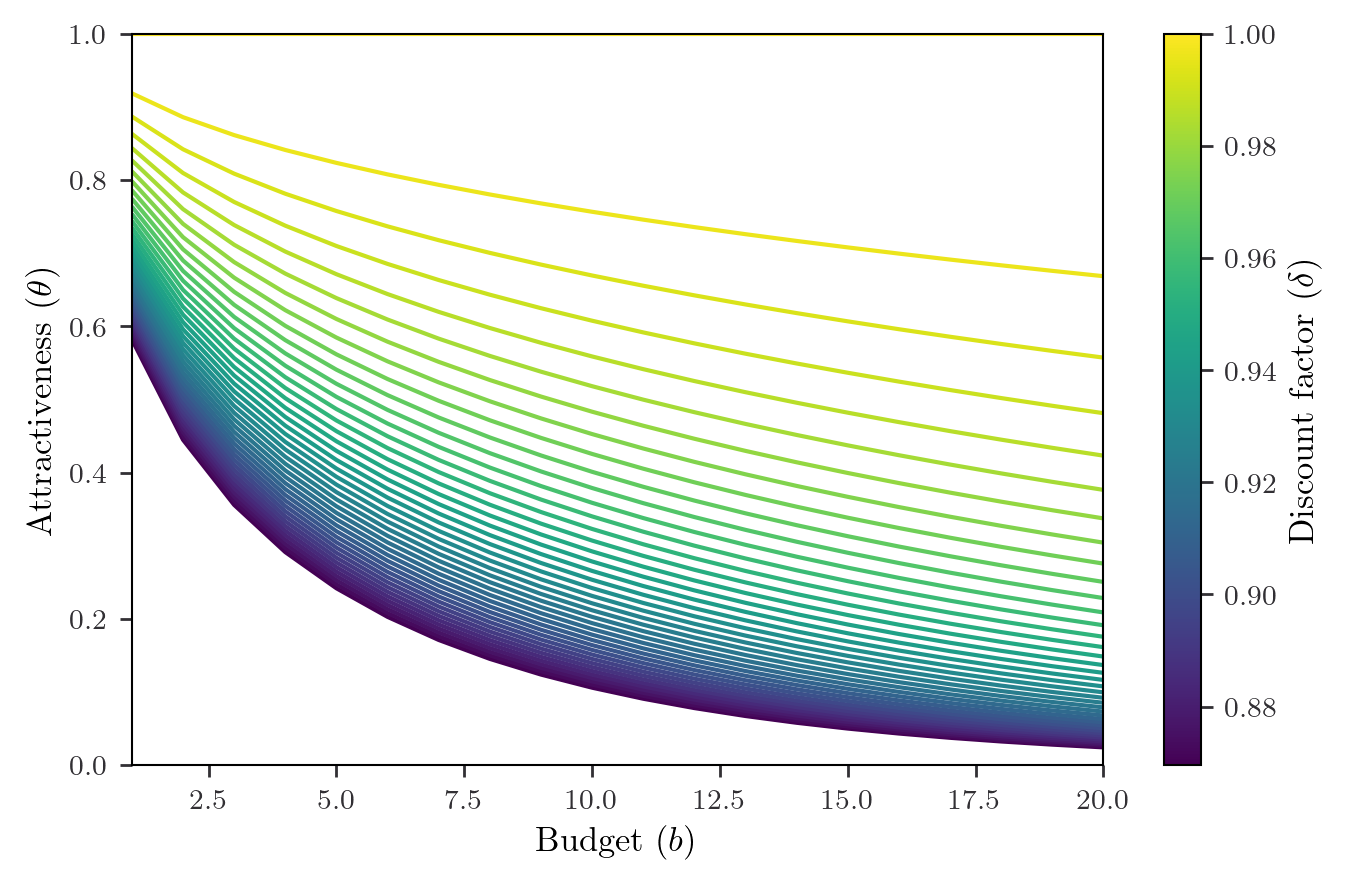
\includegraphics{discount-cs.png}
    \label{fig:discount-cs}
\end{figure} 

Another interesting parameter to examine is the absolute risk aversion of agents, which I choose to interpret as their `desperateness' for matching.
In the platform, risk-averse agents prefer a greater likelihood of matching (even if this yields relatively lower payoffs), whilst risk-loving agents prefer to save their swipes for high-yield candidates. 
To perform comparative statics on this parameter, I fix a CARA utility function for agents, with parameter $r$ corresponding to the Arrow-Pratt coefficient for absolute risk aversion. 
I then compute the optimal swiping rule for various different values of $r$, with results for this shown on \autoref{fig:risk-cs}.
From here, it is evident that as absolute risk aversion rises, agents become `more desperate' for matches, inducing them to lower their standards for right-swiping on a candidate, and thus shifting their swiping curve downwards.

\begin{figure}[ht]
    \centering
    \caption{Comparative Statics on Absolute Risk Aversion}
    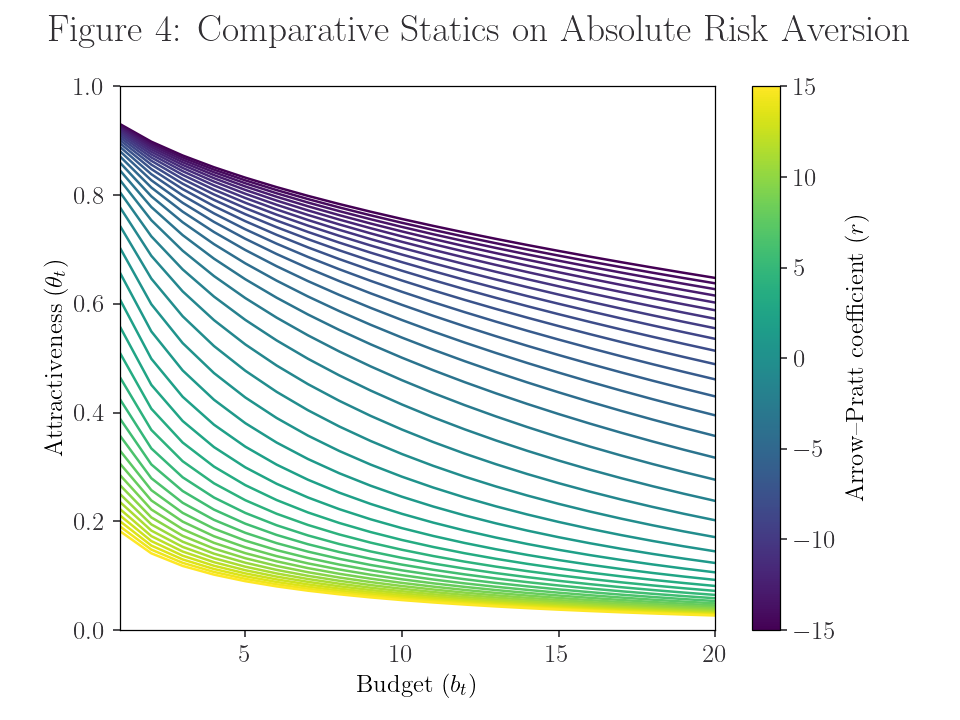
\includegraphics{risk-cs.png}
    \label{fig:risk-cs} 
\end{figure}

\subsection{Market Configuration Analysis}\label{sec:section3.3} 
Finally, I perform comparative statics at the platform level to explore how different exogenous factors affect market configurations. 
This is especially important as it considers not only the effects on best-responses for one sex, but also how these propagate across the market, ultimately affecting the other side's swiping behaviour as well. 
More specifically, I focus on the aforementioned `Fast-Swiping Men' puzzle, investigating the discrepancies in swiping rates and matching outcomes between men and women. 
There are a number of potential explanations for this behaviour, most of which concern sex-specific differential preferences which are compatible with my model. 
Indeed, it is reported that women spend around 20\% more time then men on a single Tinder session \citep{web:nytimes_patience}, potentially indicating a higher level of patience which would induce `higher standards' and a lower swiping rate, as explained above.
Departing from these, I consider below a scenario that could explain the `Fast-Swiping Men' puzzle purely as a result of tightness-induced search frictions, for which I analyse the market SE computed under a 6:1 ratio between exogenous arrival rates $\lambda_m$ and $\lambda_w$.  
This ratio was calibrated such that the steady state mass of men in the platform is around ten times greater than that of women, in line with demographic estimates for the UK \citep{web:tinder_stats}, and results for such SE are shown in \autoref{fig:mkt-cs}. 

\begin{figure}[ht]
    \centering
    \caption{Market Configuration Under Differential Agent Inflows}
    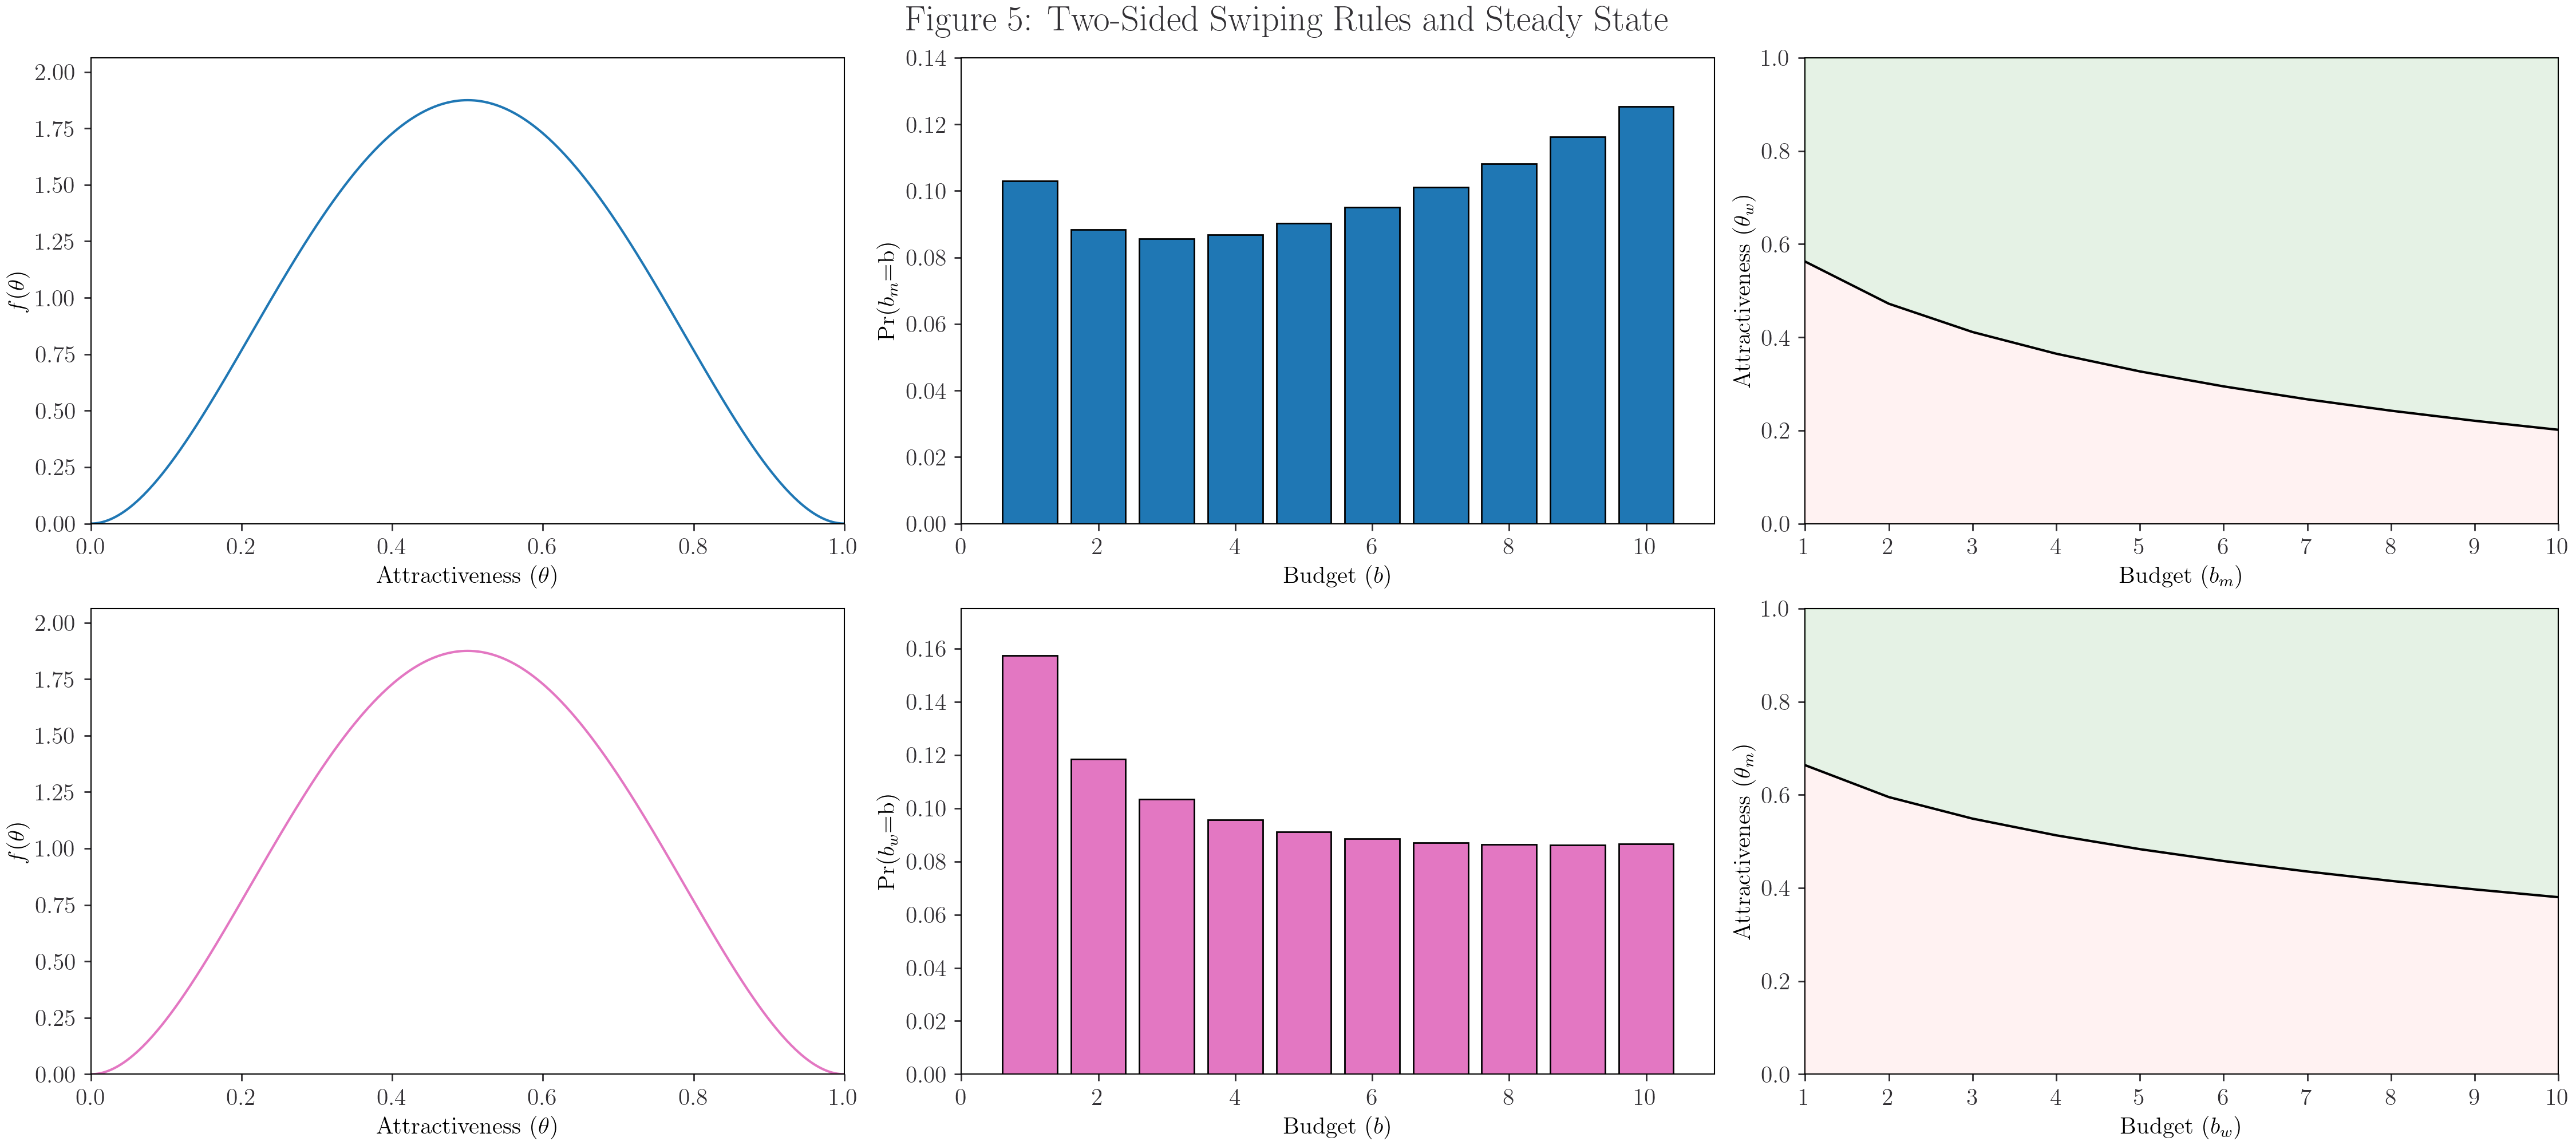
\includegraphics{mkt-cs.png}
    \label{fig:mkt-cs} 
\end{figure} 

Under the above scenario, men overcrowd the market and struggle to get paired with female candidates, as evidenced by the top-center plot in \autoref{fig:mkt-cs} which shows that male agents are highly concentrated in the top budget levels. 
Due to the effect of market tightness on the effective discount rate, male agents become more impatient than women, and this shock is absorbed by their optimal swiping policy, which sits considerably lower than the female swiping curve, effectively showing how a tight market lowers male patience and by extension, their standards, leading them to swipe right on most women. 
Ultimately, this explains the `Fast-Swiping Men' puzzle given that, under this particular SE, men swipe right with probability $\overline\mu=0.988$, compared to $\overline\omega=0.491$ for women, thus replicating the observed phenomenon. 

One potential intervention to correct this phenomenon would involve relaxing the swiping cap for the shorter side of the market.
To analyse such measure, the SE was computed under the same conditions as above but with a 4:1 swiping cap ratio between women and men; the results for this, shown in \autoref{fig:mkt-cs-bdiff}, indicate the presence of two separate effects that would help alleviate the above scenario. 
First, a larger budget set would allow women to stay in the platform for longer by shrinking the number of endogenous departures to zero (at the limit), thus leading to a larger steady state mass of female agents that would reduce market tightness for men. 
This is corroborated by the computed results, which show a 6:1 ratio between the male and female agent masses, down from 10:1. 
Furthermore, because optimal reservation values are decreasing in the agent's budget, women in the top budget levels can now swipe right at considerably lower thresholds, thus improving matching outcomes for men. 
This is highlighted in \autoref{fig:mkt-cs-bdiff}, which shows that female swiping policy quickly descends to a level comparable to its male counterpart since it is allowed to extend over a larger budget set. 
Furthermore, under this particular SE, men swipe right with probability $\overline\mu=0.906$, compared to $\overline\omega=0.79$ for women, therefore highlighting the effectiveness of this intervention, which could be of considerable importance given both its simplicity and its potential impact on user experience, as research by \cite{kanoria2021facilitating} identifies asymmetric selectiveness as a profound source of inefficiency in dynamic matching platforms. 
\begin{figure}[ht]
    \centering
    \caption{Market Configuration Under Differential Swiping Caps}
    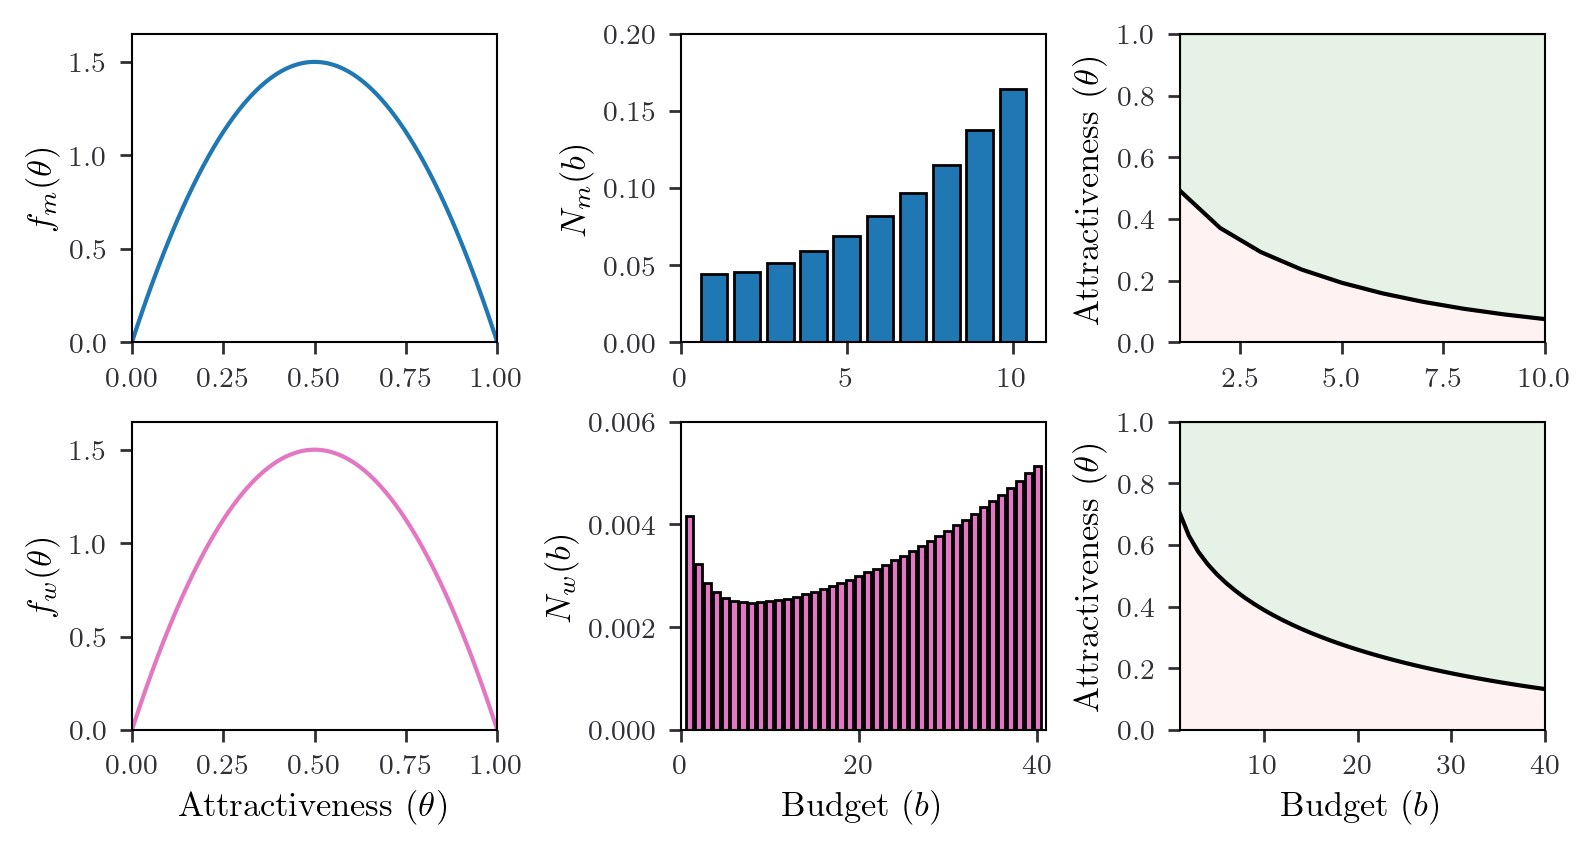
\includegraphics{mkt-cs-bdiff.png}
    \label{fig:mkt-cs-bdiff} 
\end{figure}
One potential drawback of this intervention is that general selectiveness falls in the market, since the effect prompting women to swipe more is of greater magnitude than the one prompting men to swipe less. 
This could be easily avoided by lowering the swiping cap for men, instead of raising the cap for women, to achieve the desired counterbalancing ratio, but such intervention would be inevitably bounded as the swiping cap for men approaches zero.
